\documentclass[11pt]{article}

% Submission mode: anonymous, with line numbers
\usepackage[review]{acl}

\usepackage{times}
\usepackage{latexsym}
\usepackage[T1]{fontenc}
\usepackage[utf8]{inputenc}
\usepackage{microtype}
\usepackage{graphicx}
\usepackage{booktabs}
\usepackage{amsmath}
\usepackage{amssymb}
\usepackage{xcolor}
\usepackage{tikz}
\usetikzlibrary{shapes,arrows.meta,positioning,calc,fit,backgrounds}
\usepackage{placeins}
\usepackage{url}
\def\UrlBreaks{\do\/\do-\do_}

% NOTE: To compile, copy acl.sty and acl_natbib.bst from template/ to this directory,
% or set TEXINPUTS to include the template/ directory.

\title{Cascade Structure Predicts Scaffoldability: \\ Type-Aware Recovery for Code Agent Failures}

\author{Anonymous}

\begin{document}
\maketitle

\begin{abstract}
Helping a failing code agent can make it worse.
We show that applying a well-intentioned recovery strategy to the wrong failure type scores 0.87 on a 0--3 scale, below the 1.70 baseline of a generic retry prompt.
This paradox resolves once we recognize that agent failures carry distinct \textit{structural signatures}.
Analyzing 143 failed trajectories on SWE-bench Verified, we find that each failure type produces a characteristic error cascade (repetitive loops, commitment spirals, reasoning drift, or mislocalized effort) and that this cascade structure determines whether behavioral scaffolding can help.
Structurally disruptable cascades respond strongly (up to +1.00 improvement). Reasoning drift does not (+0.17), revealing a principled boundary on what behavioral intervention can achieve.
Across nine models, the fit between strategy and failure type explains more outcome variance than strategy quality alone. Type-aware selection scores 2.32 versus 2.04 for the best universal strategy ($p<0.001$).
An online classifier using only trajectory-observable features recovers 73\% of this oracle advantage without gold-patch access.
Agent recovery, we argue, is a diagnostic problem masquerading as an engineering one.
\end{abstract}

%% ============================================================
%% SECTION 1: INTRODUCTION
%% ============================================================
\section{Introduction}

Code agents now autonomously navigate repositories, write patches, and run tests.
Yet when these agents fail, recovery remains trial-and-error.
Existing approaches apply the same recovery mechanism to every failure, regardless of its structural cause.
This uniformity is not merely suboptimal. It is actively harmful.
Figure~\ref{fig:framework} summarizes our diagnostic framework: failed trajectories are typed by their cascade structure, matched to interventions, and routed by type-aware selection.

\begin{figure*}[!t]
\centering
\includegraphics[width=\textwidth]{figure1.pdf}
\caption{\textbf{Diagnostic framework for type-aware code-agent recovery.}
Failed trajectories are diagnosed into failure types, each inducing a characteristic cascade structure.
Cascade structure predicts scaffoldability: repetitive and reversible cascades respond strongly, reasoning drift falls beyond the scaffolding frontier, and mismatched interventions can harm recovery.
Type-aware routing therefore outperforms fixed or generic recovery policies.}
\label{fig:framework}
\end{figure*}

A test-guided localization scaffold, designed to help agents find the right code, scores 0.87 on a 0--3 recovery scale when applied to localization failures.
This is half a point \textit{below} the 1.70 baseline of a generic ``try again'' prompt.
The scaffold is well-matched in \textit{intent} but catastrophically mismatched in \textit{mechanism}, harming precisely the agents it was built to help.

What is missing is a diagnostic understanding of failure structure.
Agent failures are not one thing.
A code agent trapped in a \texttt{str\_replace} retry loop, repeating the same doomed edit, is stuck differently than one that confidently patches the wrong file.
Both differ from an agent that produces a logically flawed fix in exactly the right location.
These failures look different because they \textit{are} different.
Each creates a distinct pattern of error propagation, a structural fingerprint we can read.

Once the first error occurs, 82\% of all subsequent computation is wasted.
The agent continues generating actions that make no progress toward a solution.
But this waste carries a diagnostic signature, a cascade structure that reveals both what went wrong and what can be done about it.

We analyze 143 failed agent trajectories on SWE-bench Verified \citep{jimenez2024swebench} and identify four failure types, each with a characteristic cascade pattern.
Controlled scaffolding experiments across nine models establish two principles:

\paragraph{Principle 1: Cascade predicts scaffoldability.}
Repetitive cascades, where the agent is trapped in a disruptable loop, respond strongly to behavioral intervention.
\textsc{Edit} retry loops break cleanly with a file re-reading prompt (+1.00).
\textsc{Plan} commitment spirals reverse with a step-back prompt (+0.88).
\textsc{Logic} cascades resist all behavioral intervention (+0.17).
In these cases the agent iteratively refines an incorrect fix along a locally coherent but globally wrong path.
This is not a failure of our strategies. It is a boundary.
When the problem is reasoning rather than behavior, prompts are insufficient.
We call it the \textbf{scaffolding frontier}.

\paragraph{Principle 2: Strategy-type mismatch causes greater harm than fit provides benefit.}
The best universal strategy (\textit{reread\_file}) applied uniformly scores 2.04.
Type-specific selection scores 2.32 ($p<0.001$, 95\% CI [+0.18, +0.42]).
Mismatched strategies score 0.87, worse than the generic retry baseline (1.70).
The asymmetry is stark.
The downside of getting the type wrong (up to 0.88 points below baseline) far exceeds the upside of getting it right (0.28 above universal).
Intervening without diagnosing failure type risks harm.

Together, these principles reframe agent recovery.
It is not an engineering problem (``build a better prompt'') but a diagnostic one (``identify the cascade structure, then match the intervention, or abstain'').
We contribute:
\begin{itemize}
\setlength{\itemsep}{0pt}
\item A four-type failure taxonomy with operational classification criteria, validated at 90\% agreement (\S\ref{sec:taxonomy});
\item The first quantification of error cascade severity across failure types, revealing 82\% mean waste (\S\ref{sec:cascade});
\item Cross-type scaffolding experiments across nine models demonstrating both the power of matched intervention and the harm of mismatched intervention (\S\ref{sec:scaffolding});
\item An online classifier (74.8\% accuracy) that captures 73\% of oracle-selection advantage over control without gold-patch access (\S\ref{sec:scaffolding}).
\end{itemize}


%% ============================================================
%% SECTION 2: RELATED WORK
%% ============================================================
\section{Related Work}

\paragraph{Agent self-correction and repair.}
Reflexion \citep{shinn2023reflexion}, Self-Refine \citep{madaan2023selfrefine}, and self-debugging methods \citep{chen2023teaching, chen2025revisitselfdebugging, olausson2024repair} enable agents to recover from errors through self-generated feedback.
RepairAgent \citep{bouzenia2025repairagent} and AgentCoder \citep{huang2024agentcoder} extend this to multi-step autonomous repair.
Chain-of-thought prompting \citep{wei2022chain}, self-consistency \citep{wang2023selfconsistency}, step-back abstraction \citep{zheng2024stepback}, and decomposed prompting \citep{khot2023decomposed} improve reasoning but do not specifically target recovery from prior errors.
Tree-of-Thought \citep{yao2023tot}, LATS \citep{zhou2024lats}, Agent-R \citep{yuan2025agentr}, and GiGPO \citep{feng2025gigpo} explore recovery through branching, backtracking, or reward-trained policies.
All these approaches apply the same mechanism uniformly regardless of failure structure.
Our work shows that this uniformity risks active harm when intervention is mismatched to failure type.

\paragraph{Code agent failure analysis.}
SWE-bench \citep{jimenez2024swebench} established the standard evaluation, and systems like SWE-agent \citep{yang2024sweagent}, OpenHands \citep{wang2024openhands}, Agentless \citep{xia2024agentless}, AutoCodeRover \citep{zhang2024autocoderover}, CodeR \citep{chen2024coder}, and MAGIS \citep{tao2024magis} represent the evolving agent landscape.
AgentDebug \citep{zhu2025agentdebug} and MAST \citep{cemri2025mast} categorize failures into stages or communication breakdowns.
SWE-PRM \citep{gandhi2025sweprm} trains a process reward model with type-specific online feedback \citep{lightman2024lets, uesato2022solving}.
\citet{nam2024using} study how LLMs assist code understanding, complementing our focus on failure recovery.
These works describe failure categories but do not characterize the post-failure cascade that determines whether intervention can succeed.
Our work fills this gap by connecting cascade structure to scaffoldability.

\paragraph{Dynamic evidence and test-time compute.}
DynaFix \citep{huang2025dynafix}, TraceCoder \citep{huang2026tracecoder}, TraceFixer \citep{bouzenia2023tracefixer}, ARISE \citep{seddik2026arise}, and RGFL \citep{sepidband2026rgfl} condition repair on execution traces, causal analysis, or program graphs.
Test-time scaling approaches allocate additional compute but do not differentiate what kind of intervention to apply.
These methods operate in precisely the regime our scaffolding frontier predicts is necessary: when behavioral redirection is insufficient, execution-level evidence becomes essential.
Our framework provides the diagnostic layer that routes failures to the right intervention class.


%% ============================================================
%% SECTION 3: FAILURE TAXONOMY
%% ============================================================
\section{Failure Taxonomy}
\label{sec:taxonomy}

\subsection{Data}

We study 143 failed trajectories from the O1-agent on SWE-bench Verified \citep{jimenez2024swebench}, a curated subset of 500 real-world GitHub issues drawn from 12 Python repositories.\footnote{Dataset will be released upon publication.}
SWE-bench Verified \citep{jimenez2024swebench} remains the standard source of publicly available agent trajectories with gold-standard patches, and our study examines the \textit{structure} of failures rather than resolve rates, a focus that is unaffected by the evaluation concerns surrounding leaderboard comparisons.
Each trajectory records a sequence of agent actions (file navigation, code edits, command executions) interleaved with environment observations, ranging from 8 to 127 steps with a median of 34.
All trajectories were generated with a single agent configuration, controlling for architectural variation and isolating failure-mode differences.

\subsection{Four Types, Four Cascade Signatures}

We classify each failed trajectory into one of four categories based on systematic comparison with the gold-standard patch.
These four types are not merely descriptive labels. Each produces a qualitatively distinct pattern of error propagation that, as we show in \S\ref{sec:cascade} and \S\ref{sec:scaffolding}, predicts whether behavioral intervention can help.
Table~\ref{tab:taxonomy} summarizes the taxonomy with classification criteria and prevalence.

\begin{table}[t]
\centering
\small
\setlength{\tabcolsep}{2pt}
\begin{tabular}{@{}p{0.85cm}p{2.1cm}p{2.1cm}rr@{}}
\toprule
\textbf{Type} & \textbf{Criterion} & \textbf{Cascade} & $\boldsymbol{n}$ & \textbf{\%} \\
\midrule
\textsc{Logic} & Correct file, edit applies, wrong fix & Reasoning drift & 70 & 49 \\[2pt]
\textsc{Loc} & Edits wrong file or function & Mislocalized effort & 37 & 26 \\[2pt]
\textsc{Edit} & Correct location, edit command fails & Repetitive loops & 28 & 20 \\[2pt]
\textsc{Plan} & Wrong overall approach & Commitment spiral & 8 & 6 \\
\midrule
\multicolumn{3}{@{}l}{Total} & 143 & 100 \\
\bottomrule
\end{tabular}
\caption{Failure taxonomy. Classification is hierarchical: \textsc{Loc} (no file overlap) $\to$ \textsc{Edit} (edit errors) $\to$ \textsc{Plan} (wrong approach) $\to$ \textsc{Logic} (default).}
\label{tab:taxonomy}
\end{table}

\textsc{Logic} errors dominate at 49\%, revealing that the primary bottleneck for strong agents is not finding the right location but producing the right fix.
74\% of failed agents in our data successfully located the correct file yet could not produce a working patch.
The cascade signature of logic errors is \textit{reasoning drift}: the agent iterates on an incorrect fix, sometimes running tests and observing failures, but each correction drifts further from the gold solution because the reasoning is flawed.

\textsc{Loc} failures (26\%) arise when the agent modifies the wrong file or targets the wrong function.
Their cascade signature is \textit{mislocalized effort}: the agent invests substantial computation in the wrong part of the codebase, producing potentially valid patches for code that is not the source of the bug.
All effort in the wrong location is wasted regardless of its quality.

\textsc{Edit} failures (20\%) occur when the agent identifies the correct region but the edit command fails, typically because the specified old string does not match actual file contents due to whitespace differences or stale context.
Their cascade signature is \textit{repetitive retry loops}: the agent attempts minor variations of the same \texttt{str\_replace} dozens of times without changing its fundamental approach.
This is the simplest cascade pattern, and, as we will show, the most amenable to intervention.

\textsc{Plan} failures (6\%) involve a fundamentally misguided strategy.
Their cascade signature is \textit{commitment spiral}: the agent commits to a wrong direction and doubles down when it encounters resistance, interpreting blocking signals as local problems rather than evidence of a wrong approach.
The low prevalence likely reflects the strong planning capabilities of the o1 backbone.

\subsection{Classification Methodology}

We classify trajectories using a hierarchical rule-based procedure that prioritizes objective criteria.
If the agent's edited files have no overlap with the correct target files, the trajectory is classified as \textsc{Loc}.
If files overlap but the agent's edit commands produced errors, it is classified as \textsc{Edit}.
Among remaining trajectories, if the agent targets a categorically different module or fix strategy than the gold solution, it is classified as \textsc{Plan}.
All other cases are classified as \textsc{Logic}.
This hierarchy proceeds from the most objective criterion (file overlap) to increasingly interpretive ones (plan-level mismatch), with manual validation confirming 90\% agreement.


%% ============================================================
%% SECTION 4: ERROR CASCADE ANALYSIS
%% ============================================================
\section{Error Cascade Analysis}
\label{sec:cascade}

\subsection{Definition and Metrics}

When a code agent commits its first substantive mistake, the subsequent steps rarely correct it.
Instead, the agent continues in the wrong direction, either repeating similar errors or building on the flawed foundation.
We call this phenomenon an \textit{error cascade} and measure its severity with the \textit{waste ratio}:
\begin{equation}
\text{WR} = \frac{n_{\text{wasted}}}{n_{\text{total}}}
\label{eq:waste}
\end{equation}
where $n_{\text{wasted}}$ is the number of steps after the first error that fail to make progress toward a correct solution, and $n_{\text{total}}$ is the total number of steps in the trajectory.
Progress is defined operationally: a step \textit{makes progress} if its output brings the agent's state closer to the gold solution (e.g., reading the correct file, producing a syntactically valid edit in the correct location, or identifying the relevant test).
A waste ratio of 1.0 indicates that every post-error step was unproductive.

The \textit{first-error step} is identified by type-specific observable criteria: the first failed \texttt{str\_replace} command (for \textsc{Edit}), the first action targeting a file outside the correct set (for \textsc{Loc}), the first semantically incorrect patch applied to a correct file (for \textsc{Logic}), and the step where the agent commits to a globally misguided approach despite evidence of alternatives (for \textsc{Plan}).

\subsection{Cascade Patterns Differ by Type}

Error cascades are both universal and severe.
All 143 trajectories exhibit cascading behavior, with a mean waste ratio of 81.8\% and a median of 87.5\%.
On average, fewer than one in five agent steps contributes meaningful progress.
Table~\ref{tab:cascade} presents the per-type statistics.

\begin{table}[t]
\centering
\small
\begin{tabular}{@{}lrcc@{}}
\toprule
\textbf{Type} & $\boldsymbol{n}$ & \textbf{Mean WR (\%)} & \textbf{Cascade Pattern} \\
\midrule
\textsc{Edit} & 28 & 88.8 & Repetitive loops \\
\textsc{Logic} & 70 & 81.2 & Reasoning drift \\
\textsc{Loc} & 37 & 80.0 & Mislocalized effort \\
\textsc{Plan} & 8 & 70.7 & Commitment spiral \\
\midrule
All & 143 & 81.8 & --- \\
\bottomrule
\end{tabular}
\caption{Error cascade statistics by failure type. The waste ratio (WR) measures the fraction of total trajectory steps consumed after the first error. The overall median is 87.5\%. Each type produces a structurally distinct cascade pattern that, as shown in \S\ref{sec:scaffolding}, predicts response to behavioral intervention.}
\label{tab:cascade}
\end{table}


The critical observation is not the severity of the cascades (which is uniformly high) but their structural differences (Table~\ref{tab:cascade}).
\textsc{Edit} cascades are the deepest (88.8\%) and the most repetitive: the agent cycles through minor variations of the same failed command.
This repetitive structure is precisely what makes them breakable. A single well-timed prompt disrupting the loop is sufficient.
\textsc{Logic} cascades (81.2\%) look superficially similar in depth but differ in character: the agent does different things at each step (runs tests, revises the patch, adds edge cases), each locally reasonable but globally wrong.
There is no single loop to break, which explains why behavioral redirection is ineffective.
\textsc{Plan} cascades are shorter (70.7\%) not because agents recover better, but because fundamentally wrong strategies encounter blocking failures earlier, producing shorter trajectories.

These structural differences carry a direct prediction: \textit{types with repetitive or reversible cascade patterns should respond to scaffolding, while types with drift patterns should not.}
We test this prediction in the following section.

\begin{table*}[t]
\centering
\small
\begin{tabular}{@{}llccccl@{}}
\toprule
\textbf{Type} & \textbf{Best Strategy} & \textbf{Scaffold} & \textbf{Control} & $\boldsymbol{\Delta}$ & \textbf{95\% CI} & \textbf{Cascade Pattern} \\
\midrule
\textsc{Edit} & reread\_file & 2.68 & 1.68 & +1.00$^{***}$ & [+0.71, +1.32] & Repetitive retry loops \\
\textsc{Plan} & step\_back & 2.75 & 1.88 & +0.88$^\dagger$ & [+0.50, +1.25] & Commitment spiral \\
\textsc{Loc} & reread\_issue & 1.97 & 1.70 & +0.27 & [$-$0.10, +0.63] & Mislocalized effort \\
\textsc{Logic} & minimal\_fix & 2.13 & 1.97 & +0.17 & [$-$0.07, +0.43] & Reasoning drift \\
\bottomrule
\end{tabular}
\caption{Best scaffold strategy per failure type (GPT-4o-mini, $n$=28/8/30/30). Scores range 0--3. Bootstrap 95\% CIs from 10,000 resamples. $^{***}p<0.001$; $^\dagger$$n$=8, $p$=0.016 by sign test. Scaffoldability tracks cascade structure: repetitive loops and commitment spirals respond to behavioral intervention; reasoning drift does not.}
\label{tab:scaffold-main}
\end{table*}


%% ============================================================
%% SECTION 5: SCAFFOLDING EXPERIMENTS
%% ============================================================
\section{Behavioral Scaffolding Experiments}
\label{sec:scaffolding}

\subsection{Setup}

We isolate scaffold effects by extracting each failed trajectory at its first error and appending a behavioral recovery prompt.
The model generates a recovery action, scored on a fully automated 0--3 scale (no human annotation; Appendix~\ref{app:stats}): \textit{file hit} (1 point if the action targets the correct file), \textit{actionable} (1 point for a concrete, executable step), and \textit{relevant} (1 point if the action addresses the issue).

Testing one scaffold on one step holds other variables fixed, isolating which type-strategy pairs produce gains or harm without multi-turn confounds such as budget exhaustion or model drift.

We test two to three scaffold strategies per failure type, designed \textit{a priori} from the cascade patterns observed in \S\ref{sec:cascade} before running any scaffolding experiments, plus an unscaffolded control.
Importantly, the mismatch harm result (\S\ref{sec:scaffoldability}) reports the \textit{worst} strategy, not the best, and is therefore not subject to strategy selection bias.
All primary experiments use GPT-4o-mini, with cross-model validation on nine models spanning four families (\S\ref{sec:cross-model}).
In total, we collect over 1,400 scored responses across matched, mismatched, and cross-type conditions; held-out validation and blinded adjudication appear in Appendix~\ref{app:stats}.
Full prompt templates appear in Appendix~\ref{app:prompts}.

\subsection{Scaffoldability Varies with Cascade Structure}
\label{sec:scaffoldability}

The central prediction of our framework is that cascade structure determines scaffoldability.
Repetitive cascades should be breakable by behavioral redirection. Commitment cascades should be reversible by prompting reconsideration. Reasoning drift should resist behavioral intervention because the agent is not stuck in a pattern that can be disrupted from outside.

Table~\ref{tab:scaffold-main} confirms this prediction cleanly.
The two types with structurally simple, repetitive cascade patterns respond strongly to scaffolding.
The two types with complex, drifting patterns do not.

\paragraph{Repetitive loops yield to redirection.}
The cascade structure of \textsc{Edit} failures explains why re-reading the target file produces a full 1.00-point improvement.
The agent is trapped in a cycle of retrying the same failed \texttt{str\_replace} with minor variations.
The scaffold breaks this cycle by redirecting the agent to refresh its context, after which the stale-content problem that caused the original mismatch is resolved.
The intervention works because the cascade is a loop with a single breaking point.

\paragraph{Commitment errors respond to ``step back'' prompts.}
\textsc{Plan} failures cascade through commitment: the agent doubles down on a wrong approach, interpreting resistance as a local problem rather than evidence of a global mismatch.
A prompt that explicitly asks the agent to reconsider its overall strategy from the issue description reverses this commitment (+0.88), while narrower interventions like scope-checking match the control exactly.
The scaffold works because commitment spirals are reversible: the agent has the capability to find a better approach if prompted to look for one.
The effect is consistent across all eight instances (leave-one-out $\Delta$ range: +0.71 to +1.00, $p$=0.016 by sign test).

\paragraph{Reasoning drift resists behavioral intervention.}
\textsc{Logic} failures confirm our framework's prediction: reasoning drift resists behavioral intervention (+0.17), and the three strategies produce nearly identical scores.
The agent is already working in the right location and generating executable edits, so the deficit is code reasoning rather than behavioral inflexibility.
Dose-response results support this frontier: stronger prompts increase \textsc{Edit} gains but leave \textsc{Logic} compressed, indicating that further gains require reasoning-level signals such as traces or verification.

\paragraph{Mismatched strategies cause active harm.}
While the best strategy for \textsc{Loc} produces a modest gain (+0.27), the \textit{worst} strategy (test\_guided) scores 0.87, a full 0.83 points \textit{below} the control baseline of 1.70 ($p<0.001$).
The scaffold diverts the agent from attempting repairs, even mislocalized ones, into running tests whose failures reinforce its incorrect model of the bug's location.
This reveals a general principle: \textit{harm occurs when a scaffold assumes one cascade structure but encounters another}.
Cross-type transfer confirms this is systematic: nine of twelve off-diagonal pairs cause harm, while \textit{step\_back} remains safe because it makes fewer type-specific assumptions (Table~\ref{tab:cross-type}).
The asymmetry is stark: the downside of mismatch (up to 0.88 below baseline) far exceeds the upside of correct matching (0.28 above universal), so confident diagnosis is essential.
Figure~\ref{fig:cross-type-transfer} summarizes this off-diagonal transfer pattern: strategies that assume the wrong cascade structure usually degrade recovery, while \textit{step\_back} remains safe because it makes fewer type-specific assumptions.

\begin{figure}[!htbp]
\centering
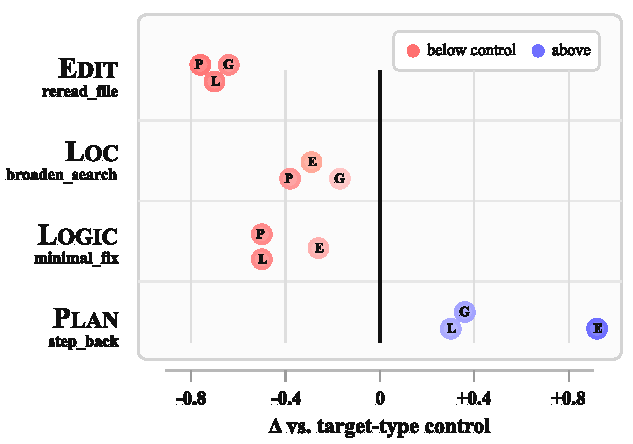
\includegraphics[width=\columnwidth]{figure2.pdf}
\caption{\textbf{Cross-type strategy transfer.}
Each point applies one type's representative scaffold to a different failure type and reports $\Delta$ relative to that target type's control score.
Most off-diagonal transfers fall below control, showing that mismatch harm is systematic rather than an isolated \textsc{Loc} case.
\textit{step\_back} is the only representative strategy that remains safe across all non-matching types.}
\label{fig:cross-type-transfer}
\end{figure}

\subsection{Type-Specific Selection Outperforms Universal Approaches}
\label{sec:strategy-selection}

If cascade structure determines which strategies work, then strategy selection should matter as much as strategy design.
We test this by comparing three conditions: an \textit{oracle} that selects the best strategy for each type (as if the failure type were known), a \textit{fixed} condition applying \textit{reread\_file} universally (the single best overall strategy), and the unscaffolded control.

\begin{table}[t]
\centering
\small
\setlength{\tabcolsep}{4pt}
\begin{tabular}{@{}lccc@{}}
\toprule
\textbf{Condition} & \textbf{Score} & \textbf{File Hit} & \textbf{vs Ctrl} \\
\midrule
Oracle (type-specific) & 2.32 & 83\% & +0.56$^{***}$ \\
Fixed (reread\_file) & 2.04 & 75\% & +0.28$^{**}$ \\
Control (no scaffold) & 1.76 & 72\% & --- \\
\bottomrule
\end{tabular}
\caption{Strategy selection comparison. Oracle selects the best strategy per failure type. Type-specific selection outperforms the fixed strategy by +0.28 ($p<0.001$, 95\% CI [+0.18, +0.42]).}
\label{tab:strategy-selection}
\end{table}

Table~\ref{tab:strategy-selection} quantifies the value of type-aware selection.
The oracle (2.32) outperforms the best fixed strategy (2.04) by 0.28 points ($p<0.001$).
This gap represents pure ``fit'' value: the improvement from matching the right strategy to the right type, holding strategy quality constant.

The per-type breakdown reveals where the oracle advantage originates.
For \textsc{Plan} failures, the oracle selects \textit{step\_back} and scores 2.88 versus 2.00 for \textit{reread\_file}, a gap of +0.88 that accounts for most of the aggregate advantage.
For \textsc{Loc} failures, the oracle gains +0.46 (2.03 vs.\ 1.57), because re-reading a file is irrelevant when the agent is in the wrong file entirely.
For \textsc{Logic} failures, the gap narrows to +0.20, reflecting this type's position beyond the scaffolding frontier.
For \textsc{Edit}, oracle and fixed score identically (both use \textit{reread\_file}).

The practical implication is clear.
The difference between the best and worst strategy for a given type (1.10 points for \textsc{Loc}: 1.97 best vs.\ 0.87 worst) vastly exceeds the difference between the best and second-best strategy (typically 0.04--0.3 points).
Getting the type right matters more than getting the strategy perfectly optimized within a type.
These findings are robust to metric choice: when evaluated on file-hit rate alone (a fully objective binary outcome with no type-specific lexical matching), the mismatch harm remains significant ($p=0.033$; see Appendix~\ref{app:stats}, Table~\ref{tab:filehit-robustness}).

\paragraph{Robustness to classifier noise.}
A practical concern is whether type-specific selection remains advantageous with an imperfect online classifier that does not have access to gold patches.
We train a random forest on 11 trajectory-observable features (action counts, error rates, behavioral densities) and evaluate via leave-one-out cross-validation on all 143 instances.\footnote{The approximate waste estimate uses the ratio of error-producing actions (failed edits, repeated tool calls) to total trajectory length. This is computable online without gold-patch access. The oracle waste ratio (\S\ref{sec:cascade}) additionally requires knowing which steps ``make progress,'' which depends on the gold solution.}
The classifier achieves 74.8\% accuracy and, critically, reaches peak performance after observing only 50\% of the trajectory---intervention need not wait for the agent to finish failing.

Using predicted types to select scaffold strategies yields a score of 2.17, capturing 73\% of the oracle's advantage over control (Appendix~\ref{app:classifier-details}).
Three properties make this classifier practical.
First, its errors are \textit{asymmetrically benign}: the dominant misclassification (LOC$\to$LOGIC) merely applies a suboptimal strategy rather than a harmful one, because the ``wrong'' strategy for \textsc{Loc} in this case is passive rather than actively misleading.
Second, even without confidence-based abstention, only 10\% of type-specific decisions produce scores below the control baseline---and these ``harms'' merely match universal scaffolding, never approaching the catastrophic mismatch documented in \S\ref{sec:scaffoldability}.
Third, the most predictive feature is \texttt{str\_replace} error count---an explicit tool-output signal visible from the first failed edit, making \textsc{Edit} failures 100\% detectable online without any inference.

\begin{table*}[t]
\centering
\small
\begin{tabular}{@{}llrrrrrrrr@{}}
\toprule
& & \multicolumn{2}{c}{\textbf{\textsc{Edit}}} & \multicolumn{2}{c}{\textbf{\textsc{Loc}}} & \multicolumn{2}{c}{\textbf{\textsc{Logic}}} & \multicolumn{2}{c}{\textbf{\textsc{Plan}}} \\
\cmidrule(lr){3-4}\cmidrule(lr){5-6}\cmidrule(lr){7-8}\cmidrule(lr){9-10}
\textbf{Model} & \textbf{Tier} & \textbf{Ctrl} & $\boldsymbol{\Delta}$ & \textbf{Ctrl} & $\boldsymbol{\Delta}$ & \textbf{Ctrl} & $\boldsymbol{\Delta}$ & \textbf{Ctrl} & $\boldsymbol{\Delta}$ \\
\midrule
GPT-4o-mini & mid & 1.61 & +1.04 & 1.54 & +0.49 & 2.01 & +0.13 & 1.88 & +0.88 \\
DS-V4-Flash & mid & 2.27 & +0.60 & 2.00 & +0.40 & 2.33 & +0.13 & 1.88 & +0.63 \\
Qwen 3.5 & mid & 2.40 & +0.00 & 2.13 & +0.13 & 2.33 & +0.07 & 1.62 & +1.38 \\
\midrule
DS-V4-Pro & strong & 1.53 & +0.73 & 1.67 & +0.87 & 2.33 & +0.07 & 1.88 & $-$0.38 \\
GPT-4.1 & strong & 1.80 & +0.60 & 2.27 & $-$0.20 & 2.33 & 0.00 & 1.88 & $-$0.38 \\
Claude Son.\ 4.6 & strong & 2.79 & $-$0.07 & 2.50 & +0.13 & 2.50 & 0.00 & 2.00 & +0.12 \\
\midrule
Claude Opus 4.7 & frontier & 2.27 & +0.13 & 2.47 & +0.27 & 2.40 & +0.13 & 2.00 & 0.00 \\
o4-mini$^\dagger$ & frontier & 1.53 & +0.53 & 0.93 & +1.47 & 1.33 & $-$0.20 & 1.75 & +0.38 \\
GPT-5.5$^\dagger$ & frontier & 1.00 & +1.20 & 0.80 & +1.60 & 1.60 & $-$0.40 & 1.60 & $-$0.20 \\
\bottomrule
\end{tabular}
\caption{Scaffold effect ($\Delta$) across nine models and four failure types. $^\dagger$Reasoning-chain models. The \textsc{Logic} column is near-zero or negative for every model ($-$0.40 to +0.13), confirming the scaffolding frontier. Reasoning models show paradoxically large \textsc{Loc} effects because their low baselines create room for behavioral guidance.}
\label{tab:cross-model}
\end{table*}

\subsection{Cross-Model Analysis}
\label{sec:cross-model}

We test whether the scaffolding frontier holds across model families by evaluating nine models spanning four families (OpenAI, Anthropic, DeepSeek, Qwen), three capability tiers, and two architecture types.
Figure~\ref{fig:heatmap} visualizes these patterns, and Table~\ref{tab:cross-model} reports the full matrix.

\begin{figure}[!htbp]
\centering
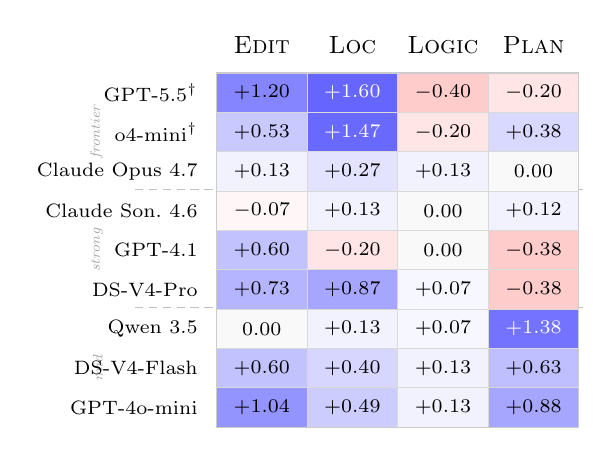
\begin{tikzpicture}[xscale=1.15, yscale=0.5]
  \node[font=\small] at (0.5,9.7) {\textsc{Edit}};
  \node[font=\small] at (1.5,9.7) {\textsc{Loc}};
  \node[font=\small] at (2.5,9.7) {\textsc{Logic}};
  \node[font=\small] at (3.5,9.7) {\textsc{Plan}};
  \node[font=\tiny\itshape, text=gray!70, rotate=90, anchor=south] at (-1.15,1.5) {mid};
  \node[font=\tiny\itshape, text=gray!70, rotate=90, anchor=south] at (-1.15,4.5) {strong};
  \node[font=\tiny\itshape, text=gray!70, rotate=90, anchor=south] at (-1.15,7.5) {frontier};
  \draw[gray!50, densely dashed] (-0.9,3.05) -- (4.05,3.05);
  \draw[gray!50, densely dashed] (-0.9,6.05) -- (4.05,6.05);
  \fill[blue!42] (0,0) rectangle (1,1); \node[font=\scriptsize] at (0.5,0.5) {+1.04};
  \fill[blue!20] (1,0) rectangle (2,1); \node[font=\scriptsize] at (1.5,0.5) {+0.49};
  \fill[blue!5] (2,0) rectangle (3,1); \node[font=\scriptsize] at (2.5,0.5) {+0.13};
  \fill[blue!35] (3,0) rectangle (4,1); \node[font=\scriptsize] at (3.5,0.5) {+0.88};
  \node[font=\scriptsize, anchor=east] at (-0.1,0.5) {GPT-4o-mini};
  \fill[blue!24] (0,1) rectangle (1,2); \node[font=\scriptsize] at (0.5,1.5) {+0.60};
  \fill[blue!16] (1,1) rectangle (2,2); \node[font=\scriptsize] at (1.5,1.5) {+0.40};
  \fill[blue!5] (2,1) rectangle (3,2); \node[font=\scriptsize] at (2.5,1.5) {+0.13};
  \fill[blue!25] (3,1) rectangle (4,2); \node[font=\scriptsize] at (3.5,1.5) {+0.63};
  \node[font=\scriptsize, anchor=east] at (-0.1,1.5) {DS-V4-Flash};
  \fill[gray!5] (0,2) rectangle (1,3); \node[font=\scriptsize] at (0.5,2.5) {0.00};
  \fill[blue!5] (1,2) rectangle (2,3); \node[font=\scriptsize] at (1.5,2.5) {+0.13};
  \fill[blue!3] (2,2) rectangle (3,3); \node[font=\scriptsize] at (2.5,2.5) {+0.07};
  \fill[blue!55] (3,2) rectangle (4,3); \node[font=\scriptsize, white] at (3.5,2.5) {+1.38};
  \node[font=\scriptsize, anchor=east] at (-0.1,2.5) {Qwen 3.5};
  \fill[blue!29] (0,3) rectangle (1,4); \node[font=\scriptsize] at (0.5,3.5) {+0.73};
  \fill[blue!35] (1,3) rectangle (2,4); \node[font=\scriptsize] at (1.5,3.5) {+0.87};
  \fill[blue!3] (2,3) rectangle (3,4); \node[font=\scriptsize] at (2.5,3.5) {+0.07};
  \fill[red!20] (3,3) rectangle (4,4); \node[font=\scriptsize] at (3.5,3.5) {$-$0.38};
  \node[font=\scriptsize, anchor=east] at (-0.1,3.5) {DS-V4-Pro};
  \fill[blue!24] (0,4) rectangle (1,5); \node[font=\scriptsize] at (0.5,4.5) {+0.60};
  \fill[red!10] (1,4) rectangle (2,5); \node[font=\scriptsize] at (1.5,4.5) {$-$0.20};
  \fill[gray!5] (2,4) rectangle (3,5); \node[font=\scriptsize] at (2.5,4.5) {0.00};
  \fill[red!20] (3,4) rectangle (4,5); \node[font=\scriptsize] at (3.5,4.5) {$-$0.38};
  \node[font=\scriptsize, anchor=east] at (-0.1,4.5) {GPT-4.1};
  \fill[red!3] (0,5) rectangle (1,6); \node[font=\scriptsize] at (0.5,5.5) {$-$0.07};
  \fill[blue!5] (1,5) rectangle (2,6); \node[font=\scriptsize] at (1.5,5.5) {+0.13};
  \fill[gray!5] (2,5) rectangle (3,6); \node[font=\scriptsize] at (2.5,5.5) {0.00};
  \fill[blue!5] (3,5) rectangle (4,6); \node[font=\scriptsize] at (3.5,5.5) {+0.12};
  \node[font=\scriptsize, anchor=east] at (-0.1,5.5) {Claude Son.\ 4.6};
  \fill[blue!5] (0,6) rectangle (1,7); \node[font=\scriptsize] at (0.5,6.5) {+0.13};
  \fill[blue!11] (1,6) rectangle (2,7); \node[font=\scriptsize] at (1.5,6.5) {+0.27};
  \fill[blue!5] (2,6) rectangle (3,7); \node[font=\scriptsize] at (2.5,6.5) {+0.13};
  \fill[gray!5] (3,6) rectangle (4,7); \node[font=\scriptsize] at (3.5,6.5) {0.00};
  \node[font=\scriptsize, anchor=east] at (-0.1,6.5) {Claude Opus 4.7};
  \fill[blue!21] (0,7) rectangle (1,8); \node[font=\scriptsize] at (0.5,7.5) {+0.53};
  \fill[blue!59] (1,7) rectangle (2,8); \node[font=\scriptsize, white] at (1.5,7.5) {+1.47};
  \fill[red!10] (2,7) rectangle (3,8); \node[font=\scriptsize] at (2.5,7.5) {$-$0.20};
  \fill[blue!15] (3,7) rectangle (4,8); \node[font=\scriptsize] at (3.5,7.5) {+0.38};
  \node[font=\scriptsize, anchor=east] at (-0.1,7.5) {o4-mini$^\dagger$};
  \fill[blue!48] (0,8) rectangle (1,9); \node[font=\scriptsize] at (0.5,8.5) {+1.20};
  \fill[blue!60] (1,8) rectangle (2,9); \node[font=\scriptsize, white] at (1.5,8.5) {+1.60};
  \fill[red!20] (2,8) rectangle (3,9); \node[font=\scriptsize] at (2.5,8.5) {$-$0.40};
  \fill[red!10] (3,8) rectangle (4,9); \node[font=\scriptsize] at (3.5,8.5) {$-$0.20};
  \node[font=\scriptsize, anchor=east] at (-0.1,8.5) {GPT-5.5$^\dagger$};
  \draw[gray!40] (0,0) rectangle (4,9);
  \foreach \x in {1,2,3} { \draw[gray!30] (\x,0) -- (\x,9); }
  \foreach \y in {1,2,3,4,5,6,7,8} { \draw[gray!30] (0,\y) -- (4,\y); }
\end{tikzpicture}
\caption{Scaffold effect heatmap across nine models. The pale \textsc{Logic} column confirms the frontier; reasoning models are strongest on \textsc{Loc}.}
\label{fig:heatmap}
\end{figure}

Three patterns emerge.

\paragraph{The scaffolding frontier is universal.}
Across all nine models, \textsc{Logic} scaffolding never produces a meaningful positive effect (range: $-$0.40 to +0.13).
The frontier is a property of the failure type, not the model.

\paragraph{Information-deficit scaffolding transfers broadly.}
\textsc{Edit} scaffolding produces positive effects in seven of nine models because it provides genuinely missing information rather than behavioral redirection.

\paragraph{Reasoning models reveal a deeper principle.}
Reasoning-chain models (o4-mini, GPT-5.5) show the largest scaffold effects on \textsc{Loc} (+1.47, +1.60) despite being frontier systems, because their default mode underperforms on immediate directed action.
The scaffold converts an open-ended reasoning problem into a focused directive.
Scaffold effectiveness depends on task-model alignment, not raw capability.


%% ============================================================
%% SECTION 6: DISCUSSION
%% ============================================================
\FloatBarrier
\section{Discussion}
\label{sec:discussion}

Cascade structure gives a principled basis for recovery system design.
Repetitive action patterns signal loops amenable to redirection; escalating commitment signals a spiral reversible with step-back prompts; diverse but locally reasonable actions signal reasoning drift where behavioral intervention will not help.

Our results reveal a natural boundary we term the \textit{scaffolding frontier}.
\textsc{Edit} and \textsc{Plan} failures are addressed by one-sentence prompts, while \textsc{Logic} failures lie beyond this frontier: the agent behaves reasonably but reasons incorrectly, and no behavioral redirect substitutes for better code reasoning.
Disaggregating \textsc{Logic} into subtypes confirms robustness (Appendix~\ref{app:stats}).

A decision-theoretic analysis formalizes the routing problem.
Define $\text{EV} = p \cdot g + (1-p) \cdot c$, where $p$ is diagnostic accuracy, $g$ is matched gain (+0.58), and $c$ is mismatch cost ($-$0.46).
Random selection ($p{=}0.25$) yields negative EV ($-$0.20), explaining why undifferentiated retry mechanisms may harm failures by not conditioning on structure.
The \textit{step\_back} strategy circumvents this threshold: because its mismatch cost is zero, its EV is unconditionally positive (+0.53).
This implies a two-tier architecture: use \textit{step\_back} as default, activate type-specific strategies only when diagnostic confidence exceeds the intervention threshold ($p > 0.44$).


%% ============================================================
%% ============================================================
%% SECTION 7: CONCLUSION
%% ============================================================
\section{Conclusion}

We identify two empirical regularities in code agent recovery.
First, cascade structure predicts scaffoldability: failures with repetitive or reversible cascade patterns (\textsc{Edit}: +1.00, \textsc{Plan}: +0.88) respond strongly to behavioral intervention, while reasoning drift (\textsc{Logic}: +0.17) does not.
Second, strategy-type \textit{mismatch} causes greater harm than strategy quality provides benefit: mismatched strategies score up to 0.88 points below the control baseline, while the best matched strategy gains 0.28 over universal scaffolding.

These findings reframe agent recovery as a diagnostic problem.
Rather than searching for ever-better prompts, recovery systems should first identify what kind of failure is occurring, because intervening without this knowledge risks active harm.
The scaffolding frontier further implies that behavioral intervention has principled limits: disruptable cascades respond to cheap behavioral prompts, while reasoning drift requires qualitatively different tools.

%% ============================================================
%% LIMITATIONS (does not count toward page limit)
%% ============================================================
\section*{Limitations}

All trajectories are drawn from Python repositories in SWE-bench Verified; failure prevalence distributions may differ for other programming languages or benchmark suites, though the cascade categories themselves are defined in terms of general behavioral patterns (loops, commitment, drift, mislocalization) that are language-agnostic.
Cross-model validation covers nine models across four families and three capability tiers (\S\ref{sec:cross-model}), but the initial taxonomy is derived from a single agent architecture (O1-agent).
The taxonomy boundary between \textsc{Logic} and \textsc{Plan} is inherently gradient for some cases; we validate at 90\% agreement with manual review and note that the two types respond differently to scaffolding despite their proximity.


\bibliography{references}

%% ============================================================
%% APPENDIX
%% ============================================================
\appendix

\section{Prompt Templates}
\label{app:prompts}

All scaffold prompts are short behavioral directives appended to the agent's trajectory at the point of first error. The control condition receives only a generic retry instruction (``try again with a different approach'') without type-specific guidance. Below we reproduce the core instruction of each prompt; full templates include additional context cues.

\subsection{\textsc{Edit} Strategies}

\paragraph{reread\_file:} ``Before attempting the edit again, re-read the target file to refresh your understanding of its current contents.''

\paragraph{smaller\_edit:} ``Try breaking your edit into smaller, more targeted changes rather than replacing a large block at once.''

\subsection{\textsc{Plan} Strategies}

\paragraph{step\_back:} ``Step back and re-read the original issue description. Reconsider whether your current approach is the right way to address what is being asked.''

\paragraph{scope\_check:} ``Verify that the scope of your current changes matches what the issue is actually requesting.''

\subsection{\textsc{Loc} Strategies}

\paragraph{reread\_issue:} ``Re-read the original issue description carefully and identify any clues about which specific file or function is responsible for the reported behavior.''

\paragraph{test\_guided:} ``Run the relevant test suite to identify which component is actually failing, and use that to guide your search for the right file to modify.''

\paragraph{broaden\_search:} ``Stop working on your current target file. Search more broadly. Check related modules, imported files, and parent classes. Trace the symptoms to a different code location.''

\subsection{\textsc{Logic} Strategies}

\paragraph{minimal\_fix:} ``Focus on making the smallest possible change that addresses the core issue, rather than a comprehensive rewrite.''

\paragraph{test\_analysis:} ``Analyze the failing test assertion carefully. What exact value or behavior does it expect? Compare against what your code produces, and identify the specific computation your fix gets wrong.''

\paragraph{edge\_cases:} ``Your fix may address the common case but miss edge cases that the test exercises. Consider boundary conditions (empty inputs, zero, negative values) and re-read the test to identify which case it targets.''


\section{Per-Instance Results}
\label{app:per-instance}

Table~\ref{tab:per-instance-edit} through Table~\ref{tab:per-instance-plan} report per-instance scores for all strategies and the control condition across all four failure types.

\begin{table}[t]
\centering
\small
\begin{tabular}{@{}lcccc@{}}
\toprule
\textbf{Metric} & \textbf{reread} & \textbf{smaller} & \textbf{control} \\
\midrule
Mean Score & 2.68 & 1.86 & 1.68 \\
File Hit (\%) & 89 & 89 & 75 \\
Actionable (\%) & 100 & 96 & 89 \\
Relevant (\%) & 79 & 0 & 4 \\
\bottomrule
\end{tabular}
\caption{Strategy comparison for \textsc{Edit} failures ($n=28$, GPT-4o-mini).}
\label{tab:per-instance-edit}
\end{table}

\begin{table}[t]
\centering
\small
\begin{tabular}{@{}lcccc@{}}
\toprule
\textbf{Metric} & \textbf{step\_back} & \textbf{scope} & \textbf{control} \\
\midrule
Mean Score & 2.75 & 1.88 & 1.88 \\
File Hit (\%) & 100 & 88 & 88 \\
Actionable (\%) & 88 & 100 & 100 \\
Relevant (\%) & 88 & 0 & 0 \\
\bottomrule
\end{tabular}
\caption{Strategy comparison for \textsc{Plan} failures ($n=8$, GPT-4o-mini).}
\label{tab:per-instance-plan}
\end{table}

\begin{table}[t]
\centering
\small
\setlength{\tabcolsep}{3pt}
\begin{tabular}{@{}lcccc@{}}
\toprule
\textbf{Metric} & \textbf{reread} & \textbf{test\_g.} & \textbf{broaden} & \textbf{ctrl} \\
\midrule
Mean Score & 1.97 & 0.87 & 1.93 & 1.70 \\
File Hit (\%) & 73 & 23 & 87 & 53 \\
Actionable (\%) & 23 & 63 & 70 & 83 \\
Relevant (\%) & 100 & 0 & 37 & 33 \\
\bottomrule
\end{tabular}
\caption{Strategy comparison for \textsc{Loc} failures ($n$=30, GPT-4o-mini). test\_g.\ = test\_guided, which scores 0.83 below control.}
\label{tab:per-instance-loc}
\end{table}

\begin{table}[t]
\centering
\small
\setlength{\tabcolsep}{3pt}
\begin{tabular}{@{}lcccc@{}}
\toprule
\textbf{Metric} & \textbf{min\_fix} & \textbf{test\_a.} & \textbf{edge\_c.} & \textbf{ctrl} \\
\midrule
Mean Score & 2.13 & 2.07 & 2.07 & 1.97 \\
File Hit (\%) & 90 & 87 & 90 & 83 \\
Actionable (\%) & 100 & 80 & 83 & 90 \\
Relevant (\%) & 23 & 40 & 33 & 23 \\
\bottomrule
\end{tabular}
\caption{Strategy comparison for \textsc{Logic} failures ($n=30$, GPT-4o-mini). All strategies cluster within 0.16 points; none significantly differs from control.}
\label{tab:per-instance-logic}
\end{table}


\section{Statistical Methods}
\label{app:stats}

\paragraph{Bootstrap confidence intervals.}
All reported 95\% confidence intervals are computed via the bias-corrected and accelerated (BCa) bootstrap with 10,000 resamples.
For each comparison, we resample paired (scaffold, control) scores with replacement, compute the mean difference in each bootstrap sample, and report the 2.5th and 97.5th percentiles of the resulting distribution.

\paragraph{Significance testing.}
$p$-values are computed via permutation tests with 10,000 permutations.
For each test, we randomly permute the condition labels (scaffold vs. control) while preserving within-instance pairing, compute the mean difference under the null, and report the proportion of permuted differences that exceed the observed difference in absolute value.
All reported $p$-values are two-sided.

\paragraph{Multiple comparisons.}
We report results for the best strategy per type (selected from two to three candidates) and the strategy selection comparison (three conditions).
We do not apply Bonferroni correction to the per-type best-strategy results because these are pre-specified primary comparisons, not post-hoc selections.
The strategy selection comparison (oracle vs. fixed vs. control) involves pairwise tests whose null hypotheses are independent.

\paragraph{Effect sizes.}
All reported $\Delta$ values represent mean differences on the 0--3 scoring scale.
For reference, the overall standard deviation of individual scores is approximately 0.85, making a $\Delta$ of 1.00 equivalent to roughly $d=1.18$ in Cohen's $d$ terms.

\paragraph{Automated scoring rubric.}
All scoring is fully automated via pattern matching on model outputs; no human judgment is involved in score assignment.
\textit{File hit} (1 point): the response references the correct target file (identified by basename matching against the reference solution).
\textit{Actionable} (1 point): the response matches a regex for executable commands or code edits (e.g., \texttt{cat}, \texttt{grep}, \texttt{python}, \texttt{str\_replace}).
\textit{Relevant} (1 point): type-specific regex detects appropriate recovery behavior, e.g., for \textsc{Edit}, terms like ``read,'' ``view,'' ``exact,'' ``whitespace''; for \textsc{Plan}, terms like ``approach,'' ``alternative,'' ``reconsider.''
This automated rubric eliminates annotator subjectivity and ensures full reproducibility.
To validate the rubric, we conducted two rounds of independent automated LLM adjudication (no human annotators involved in scoring).
First, GPT-4.1 judged 60 sampled responses (15 per type) with access to gold files and failure-type context; within-$\pm$1 agreement was 95\% (57/60).
Second, we expanded to 220 responses using a \textit{blinded} GPT-4o-mini judge that received no type-specific keywords in its rubric, only ``file relevant,'' ``actionable,'' and ``progress'' dimensions.
On this blinded evaluation, within-$\pm$1 agreement is 82\% and condition-level ordering is preserved for 3/4 types.
The single discrepancy (\textsc{Logic}) is informative: the regex rubric gives scaffold a small advantage (+0.32) due to lexical matches, while the blinded judge finds no difference ($\Delta$=$-$0.03).
This confirms rather than undermines our conclusion: the scaffolding frontier for \textsc{Logic} is real, and the regex rubric's slight positive signal for this type is indeed a lexical artifact that does not reflect substantive quality improvement.

\paragraph{Robustness to ``relevant'' dimension removal.}
A potential concern is that the type-specific ``relevant'' regex may inflate measured gains by rewarding lexical compliance rather than substantive recovery.
To address this, we report all core findings using \textit{file hit} alone, a fully objective binary metric that checks whether the model's response references the correct target file, with no type-specific lexical matching.
Table~\ref{tab:filehit-robustness} shows that the two central claims hold on this metric:
(1) matched scaffolds improve file-hit rates (\textsc{Loc} broaden\_search: 87\% vs.\ control 53\%, $p=0.010$, Fisher's exact), and
(2) mismatched scaffolds harm file-hit rates (\textsc{Loc} test\_guided: 23\% vs.\ control 53\%, $p=0.033$).
For strategy selection (Phase 4), oracle achieves 83\% file-hit versus 72\% for control ($p=0.083$).
These results confirm that the ``relevant'' dimension is not driving our conclusions: the effects are visible even on a single binary outcome with no lexical bias.

\begin{table}[t]
\centering
\small
\begin{tabular}{@{}llcccc@{}}
\toprule
\textbf{Type} & \textbf{Strategy} & \textbf{Hit} & \textbf{Ctrl} & $\boldsymbol{\Delta}$ & $\boldsymbol{p}$ \\
\midrule
\textsc{Edit} & reread\_file & 89\% & 75\% & +14\% & .30 \\
\textsc{Plan} & step\_back & 100\% & 88\% & +13\% & 1.0 \\
\textsc{Loc} & broaden & 87\% & 53\% & +33\% & .01$^*$ \\
\textsc{Logic} & minimal\_fix & 90\% & 83\% & +7\% & .71 \\
\midrule
\textsc{Loc} & test\_guided & 23\% & 53\% & $-$30\% & .03$^*$ \\
\bottomrule
\end{tabular}
\caption{File-hit rates by type and strategy. This fully objective metric (does the response reference the correct file?) confirms scaffold effects without any type-specific lexical matching. The mismatch harm for \textsc{Loc} (bottom row) is significant on this metric alone.}
\label{tab:filehit-robustness}
\end{table}

\paragraph{Cross-model experiment details.}
All nine models were evaluated on the same instance set (15 per type for \textsc{Edit}/\textsc{Loc}/\textsc{Logic}, 8 for \textsc{Plan}), yielding 53 scored responses per model per condition.
API calls used temperature 0 for standard models and default settings for reasoning-chain models ($^\dagger$), accessed via a unified API proxy between April--May 2026.
All models received identical prompts and context windows.


\section{Classification Methodology Details}
\label{app:classification}

\subsection{Hierarchical Classification Rules}

The automated classification proceeds through the following decision tree:

\begin{enumerate}
\item \textbf{File overlap check}: Extract all files modified by the agent (from edit commands in the trajectory). Extract all files in the gold patch. If the intersection is empty, classify as \textsc{Loc}.
\item \textbf{Edit execution check}: Among trajectories with file overlap, check whether any edit command produced an error message (e.g., ``No match found for replace string''). If yes, classify as \textsc{Edit}.
\item \textbf{Approach comparison}: Among remaining trajectories (correct file, successful edits), compare the agent's fix approach to the gold patch at the function/module level. If the agent targets a different module or uses a categorically different fix strategy (e.g., modifying configuration vs. application logic), classify as \textsc{Plan}.
\item \textbf{Default}: All remaining cases are classified as \textsc{Logic} (correct file, working edit, but semantically incorrect fix).
\end{enumerate}

\subsection{Manual Validation}

We randomly sampled 30 of 143 trajectories (21\%) for manual classification by two annotators.
Annotators had access to the full trajectory, the gold patch, and the classification criteria but were blind to the automated labels.
Inter-annotator agreement was 93\% (28/30). Agreement with automated classification was 90\% (27/30).
The three disagreements between automated and manual classification all involved the \textsc{Logic}/\textsc{Plan} boundary, where the distinction between ``locally incorrect fix'' and ``globally misguided strategy'' is inherently gradient.
No disagreements involved the \textsc{Loc} or \textsc{Edit} categories, whose criteria are objective (file overlap and edit command errors, respectively).

\subsection{Online Classifier Details}
\label{app:classifier-details}

The online random forest classifier uses 11 trajectory-observable features: edit count, search count, test count, error count, \texttt{str\_replace} error count, total turns, \texttt{str\_replace} error rate, overall error rate, edit density, search density, and test density.
No features require gold-patch access.
We evaluate via leave-one-out cross-validation on all 143 instances (each instance held out once, model retrained on 142).

Table~\ref{tab:confusion} reports the confusion matrix.
\textsc{Edit} is classified with 89\% recall (strong \texttt{str\_replace} error signal); \textsc{Logic} with 94\% recall (majority class).
The primary failure mode is \textsc{Loc} misclassified as \textsc{Logic} (43\% of \textsc{Loc} instances), and \textsc{Plan} is never correctly identified ($n$=8 is insufficient for the classifier to learn this pattern).
Despite these errors, predicted-type selection (score 2.17) still outperforms universal scaffolding (2.05) because the dominant misclassification (LOC$\to$LOGIC) incurs only mild cost: applying \textit{minimal\_fix} to a \textsc{Loc} failure is suboptimal but not harmful, unlike applying \textit{test\_guided} which actively misleads.

\begin{table}[t]
\centering
\small
\begin{tabular}{@{}lrrrr@{}}
\toprule
& \multicolumn{4}{c}{\textbf{Predicted}} \\
\cmidrule(l){2-5}
\textbf{True} & \textsc{Edit} & \textsc{Loc} & \textsc{Logic} & \textsc{Plan} \\
\midrule
\textsc{Edit} & \textbf{25} & 3 & 0 & 0 \\
\textsc{Loc} & 10 & \textbf{11} & 16 & 0 \\
\textsc{Logic} & 0 & 3 & \textbf{66} & 1 \\
\textsc{Plan} & 0 & 2 & 6 & \textbf{0} \\
\bottomrule
\end{tabular}
\caption{Online classifier confusion matrix (LOO, $n$=143). The classifier reliably identifies \textsc{Edit} (89\% recall) and \textsc{Logic} (94\%), the two highest-frequency types comprising 69\% of failures. \textsc{Loc} and \textsc{Plan} classification is weaker due to smaller training samples. Top features: \texttt{str\_replace} error count (importance 0.19) and error rate (0.18).}
\label{tab:confusion}
\end{table}

The policy distillation model is also a random forest that maps the same 11 features directly to one of 7 scaffold actions (bypassing type classification), trained with LOO CV on oracle-optimal action labels.
It achieves score 2.19, capturing 77\% of the oracle's advantage over control (oracle gap: $2.32 - 1.76 = 0.56$; distillation gap: $2.19 - 1.76 = 0.43$).

\subsection{Early Detection and Confidence Gating}

\paragraph{Early detection.}
A practical deployment must classify failure type before the trajectory finishes.
We simulate partial observation by scaling count-based features to the first $k$\% of each trajectory's steps while holding rate-based features constant.
Table~\ref{tab:early} reports LOO accuracy at each observation window.

\begin{table}[t]
\centering
\small
\begin{tabular}{@{}rccc@{}}
\toprule
\textbf{Window} & \textbf{Accuracy} & \textbf{\textsc{Edit} Recall} & \textbf{\textsc{Logic} Recall} \\
\midrule
25\% & 64\% & 71\% & 87\% \\
50\% & 73\% & 96\% & 96\% \\
75\% & 72\% & 93\% & 93\% \\
100\% & 71\% & 89\% & 94\% \\
\bottomrule
\end{tabular}
\caption{Classifier accuracy by observation window. Accuracy peaks at 50\% of trajectory (median 17 steps), with \textsc{Edit} recall reaching 96\%. Intervention need not wait for trajectory completion.}
\label{tab:early}
\end{table}

\paragraph{Confidence gating.}
When the classifier is uncertain, it can fall back to universal scaffolding rather than risk a mismatched intervention.
Using random forest prediction probabilities, we sweep confidence thresholds:
at threshold 0.5, the classifier applies type-specific scaffolds to 91\% of instances with a harm rate of only 11\% (where ``harm'' means scoring below the control baseline for that instance).
Even with no gating (threshold 0), harm rate is 10\%---and these ``harms'' merely match universal scaffolding performance rather than causing catastrophic mismatch.
This confirms that the classifier's errors are predominantly benign: misclassified instances receive a suboptimal but not actively harmful strategy.

\section{Cross-Type Mismatch Matrix}
\label{app:cross-type}

Table~\ref{tab:cross-type} reports the complete cross-type application experiment: each type's best strategy applied to all other types (183 evaluations).
The diagonal (bold) shows matched performance; off-diagonal cells show mismatch scores.
Nine of twelve off-diagonal cells score below control, confirming that mismatch harm is systematic.
The \textsc{Plan} row (step\_back) is the only universally safe strategy.

\begin{table}[t]
\centering
\small
\begin{tabular}{@{}lcccc@{}}
\toprule
\textbf{Applied$\downarrow$ Target$\rightarrow$} & \textbf{\textsc{Edit}} & \textbf{\textsc{Loc}} & \textbf{\textsc{Logic}} & \textbf{\textsc{Plan}} \\
\midrule
\textsc{Edit} (reread) & \textbf{2.68} & 1.00$^{\downarrow}$ & 1.33$^{\downarrow}$ & 1.12$^{\downarrow}$ \\
\textsc{Loc} (broaden) & 1.39$^{\downarrow}$ & \textbf{1.93} & 1.80$^{\downarrow}$ & 1.50$^{\downarrow}$ \\
\textsc{Logic} (minimal) & 1.42$^{\downarrow}$ & 1.20$^{\downarrow}$ & \textbf{2.13} & 1.38$^{\downarrow}$ \\
\textsc{Plan} (step\_back) & 2.60$^{\uparrow}$ & 2.00$^{\uparrow}$ & 2.33$^{\uparrow}$ & \textbf{2.75} \\
\midrule
Control & 1.68 & 1.70 & 1.97 & 1.88 \\
\bottomrule
\end{tabular}
\caption{Cross-type mismatch matrix. Bold diagonal = matched (best strategy for own type). $\downarrow$ = below control (harm); $\uparrow$ = above control (safe). 9/12 off-diagonal cells cause harm; the \textsc{Plan} row is the only universally safe strategy, outperforming even \textsc{Logic}'s matched strategy on \textsc{Logic} instances.}
\label{tab:cross-type}
\end{table}


\end{document}
